\chapter{Markov chain Monte Carlo (MCMC)}

As seen from the previous part, observables of many-body systems embody a rich variety of physical phenomena emerged from statistics of microscopic configurations. Their exponentially large configuration spaces prohibit exact enumerations, and motivate us to use numerical approximation methods in the studies of their properties. In this part, we first review the traditional methods of Markov chain Monte Carlo (MCMC) and variational Monte Carlo (VMC) for classical systems, list the previously used ansatzes to approximate the Boltzmann distribution, and discuss their limitations. Then we introduce the autoregressive models with the advantage of exact sampling, and combine the strengths of the exact sampling and the Markov chain sampling to remove the bias in VMC.

When studying an observable of a classical many-body system in \cref{eq:cl-obs}, it consists of a summation over all configurations of the system, which costs an exponentially large amount of computation if performed exactly by enumeration. To obtain the result within a practical computation budget, a general method is to generate many random samples of configuration $\{\vs^{(1)}, \vs^{(2)}, \ldots, \vs^{(M)}\}$ following the target distribution $p(\vs)$, where $M$ is the sample size, and estimate the $p$-weighted summation over all configurations by the uniform average over the samples:
\begin{equation}
\bbE_\text{MC}[O] = \frac{1}{M} \sum_{i = 1}^M O\left( \vs^{(i)} \right).
\label{eq:monte-carlo}
\end{equation}
This method is named Monte Carlo, after the casino that would later become famous to every computational physicist~\cite{metropolis1949monte, landau2021guide1}. It is proved that~\cite{feller1968extention}
\begin{equation}
\Var\big[ \bbE_\text{MC}[O] \big] = \frac{1}{M} \Var[\bar{O}],
\label{eq:monte-carlo-var}
\end{equation}
where the sample variance $\Var\big[ \bbE_\text{MC}[O] \big] = \bbE_\text{MC}\left[ \left( O - \bbE_\text{MC}[O] \right)^2 \right]$ and the true variance $\Var[\bar{O}] = \overline{(O - \bar{O})^2}$. Therefore, the sample variance vanishes and the estimator converges to the true value as $M$ increases, given that the true variance is finite, and the samples are independently drawn from the true distribution.

However, generating random samples from a given distribution is not always straightforward. In computational physics, the so-called ``random numbers'' are produced by pseudorandom number generators (PRNG)~\cite{press2007numerical}, which are originally designed to generate statistically random values from the uniform distribution $\calU$ over an interval, such as $[0, 1)$. In some cases, we can transform every sample from the PRNG to a sample following the target distribution in a deterministic way: Univariate distributions can be sampled by transforming the probability density function (PDF) with a change of variable $p(x) = q(y) \frac{\partial y}{\partial x}$, also known as reparameterization, where $p(x)$ is the target distribution and $q(y)$ is the uniform distribution $\calU[0, 1)$. Multivariate distributions can be sampled by first generating multiple independent values from $\calU[0, 1)$ and then changing the variables. For example, the 2D unit Gaussian distribution
$p(x, y) = \frac{1}{2 \pi} \rme^{-\frac{1}{2} (x^2 + y^2)}$ can be sampled by the Box--Muller transform~\cite{box1958note}:
\begin{gather}
p(x, y) = q(u) q(v) \begin{Vmatrix}
\frac{\partial u}{\partial x} & \frac{\partial u}{\partial y} \\
\frac{\partial v}{\partial x} & \frac{\partial v}{\partial y}
\end{Vmatrix}, \label{eq:reparam} \\
x = r \cos \theta, \quad y = r \sin \theta, \\
r = \sqrt{-2 \ln u}, \quad \theta = 2 \pi v,
\end{gather}
where $u$ and $v$ are independently sampled from $\calU[0, 1)$, and $\lVert \cdot \rVert$ denotes the absolute value of the determinant of the matrix. Discrete distributions can be obtained by discretizing continuous distributions. For example, the Bernoulli distribution $p(x) = (1 - p_1) \delta_{x, 0} + p_1 \delta_{x, 1}$ with the parameter $p_1$ can be sampled by \cref{alg:bernoulli}. In this thesis, we refer to this kind of sampling methods as exact sampling.

\begin{algorithm}[H]
\caption[Discrete Bernoulli distribution from continuous uniform distribution]{
Discrete Bernoulli distribution from continuous uniform distribution.
}
\label{alg:bernoulli}
\begin{algorithmic}[1]
\STATE Sample $u$ from $\calU[0, 1)$
\IF{$u < p_1$}
    \STATE Output $x = 0$, $p(x) = 1 - p_1$
\ELSE
    \STATE Output $x = 1$, $p(x) = p_1$
\ENDIF
\end{algorithmic}
\end{algorithm}

In the case of Boltzmann distributions for many-body systems with complicated energy landscapes, such analytical transformation is generally impossible to find, and we can only resort to indirect methods for sampling these distributions. A common method is to construct a Markov chain of samples, whose equilibrium distribution converges to the target one, therefore this sampling method is known as Markov chain Monte Carlo (MCMC)~\cite{gelfand1990sampling, robert2020markov}. For spin systems, such a Markov chain is usually constructed by the Metropolis--Hastings algorithm~\cite{hastings1970monte}. In each sampling step, we propose to update the current configuration $\vs$ to a new one $\vs'$ with the proposal distribution $g(\vs' \mid \vs)$, where $\sum_{\vs'} g(\vs' \mid \vs) = 1$ for all $\vs$. Then we accept $\vs'$ to become the current configuration by an acceptance probability defined by
\begin{equation}
A(\vs \to \vs') = \min\left( 1, \frac{p(\vs') g(\vs \mid \vs')}{p(\vs) g(\vs' \mid \vs)} \right).
\label{eq:metropolis}
\end{equation}
Otherwise, we reject it and rollback to $\vs$. It can be checked that the target distribution $p(\vs)$ is exactly the equilibrium distribution of the Markov transition matrix:
\begin{gather}
M_{\vs_j \vs_i} = A(\vs_i \to \vs_j) g(\vs_j \mid \vs_i), \label{eq:markov-matrix} \\
\sum_{\vs_i} M_{\vs_j \vs_i} p(\vs_i) = p(\vs_j).
\end{gather}
If we want to sample the target distribution using a single Markov chain, the proposal distribution must be ergodic, which allows the initial configuration to transition to all configurations in a finite number of samples. The simplest method to propose the update is to randomly select a spin and flip it, therefore $g(\vs' \mid \vs) = g(\vs \mid \vs')$ for all $\vs$ and $\vs'$, and \cref{eq:metropolis} simplifies to
\begin{equation}
A(\vs \to \vs') = \min\left( 1, \frac{p(\vs')}{p(\vs)} \right).
\end{equation}
More advanced choices of $g(\vs' \mid \vs)$ will be discussed in \cref{sec:importance-sampling}.

When $p(\vs)$ is the Boltzmann distribution in \cref{eq:boltzmann}, the acceptance probability further simplifies to
\begin{equation}
A(\vs \to \vs') = \min\left( 1, \rme^{\,\beta \left( H(\vs) - H(\vs') \right)} \right).
\end{equation}
It avoids computing the partition function $Z$, which consists of a summation over exponentially many configurations. In the case of locally interacting systems, such as \cref{eq:cl-ising-nnn}, the energy difference of flipping a spin $s_i$ simplifies to
\begin{equation}
H(\vs) - H(\vs') = 2 s_i \left( \sum_{\text{$j$ that interacts with $i$}} J_{i j} s_j \right),
\end{equation}
so the time to compute the acceptance probability, and therefore the total time of a sampling step to propose and accept a sample, only depends on the number of neighbors interacting with a site, rather than the whole system size. This advantage makes MCMC a feasible method to study large systems.

After collecting many samples from the Markov chain, we estimate the observables using \cref{eq:monte-carlo}. Care should be taken when generating these samples, as we will discuss below.

\section{Autocorrelation time and critical slowing down}

\begin{figure}[htb]
\centering
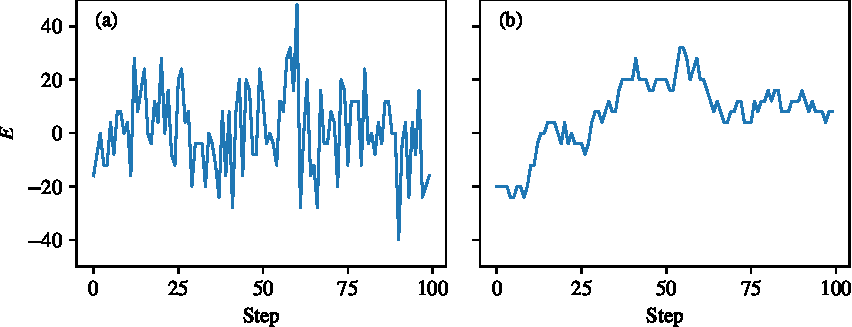
\includegraphics[width=\linewidth]{ch3/rand_autocorr.pdf}
\caption[Energy of Ising model from independent and autocorrelated samples]{
Energies of $100$ samples for the Ising model on the $10 \times 10$ square lattice.
(a) The samples are independently generated from the uniform distribution.
(b) The samples are generated by single-spin updates with $\beta = 0$.
}
\label{fig:rand-autocorr}
\end{figure}

Although MCMC allows us to estimate the observables with complicated distributions, it breaks the assumption of \cref{eq:monte-carlo} that the samples should be independent. In each sampling step, we propose a new configuration $\vs'$ that depends on the current configuration $\vs$, such as flipping a single spin. Moreover, we may reject $\vs'$ and keep using $\vs$ to evaluate the observable for this step. The visual difference between a sequence of independent samples and a Markov chain is shown in \cref{fig:rand-autocorr}. Quantitatively, the samples in the Markov chain $\{\vs^{(1)}, \vs^{(2)}, \ldots, \vs^{(M)}\}$ produce autocorrelation in the observable values~\cite{muller1973dynamic}:
\begin{equation}
C_{O, M}(t) = \left( \frac{1}{M - t} \sum_{i = 1}^{M - t} O\left( \vs^{(i)} \right) O\left( \vs^{(i + t)} \right) \right) - \bbE_\text{MCMC}^2[O],
\end{equation}
where $\bbE_\text{MCMC}[O]$ has the same form as \cref{eq:monte-carlo}, and we consider the large sample size limit
\begin{equation}
C_O(t) = \lim_{M \to \infty} C_{O, M}(t).
\end{equation}
The correlated samples cause $C_O(t) \neq 0$ when $t > 0$. For example, \cref{fig:autocorr} shows the autocorrelation in energy $C_E(t)$ of the $10 \times 10$ Ising model. As the number of steps $t$ between two samples increases, the average autocorrelation between the two samples decays to zero. At the critical temperature $\beta_\text{c} = \frac{1}{2} \ln(1 + \sqrt{2}) \approx 0.44$, the autocorrelation decays particularly slowly, and we can only assume that a sample is independent of the original one after as many as approximately $10^4$ steps, which renders the MCMC sampling inefficient.

\begin{figure}[htb]
\centering
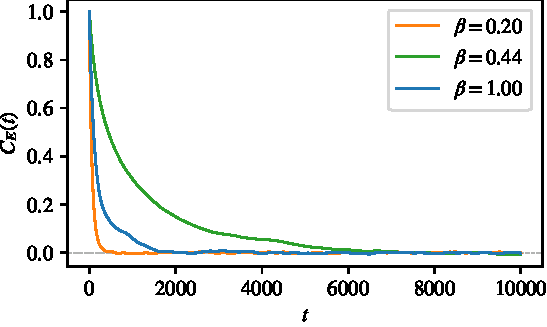
\includegraphics[width=0.6\linewidth]{ch3/autocorr.pdf}
\caption[Autocorrelation in energy of Ising model at different temperatures]{
Autocorrelation in energy $C_E(t)$ of the Ising model on the $10 \times 10$ square lattice at different inverse temperatures $\beta$. The samples are generated by single-spin updates, and the autocorrelation is estimated using $10^7$ samples.
}
\label{fig:autocorr}
\end{figure}

The integrated autocorrelation time~\cite{ambegaokar2010estimating, goodman2010ensemble}, or ``autocorrelation time'' for short, is a metric for MCMC to assess the loss in sample diversity due to autocorrelation, defined by
\begin{equation}
\tau = \frac{1}{C_O(0)} \sum_{t = 1}^\infty C_O(t).
\label{eq:iat}
\end{equation}
It depends on the complexity of the target distribution, and the method to propose new configurations. In the analytical study of the spin dynamics, it is also known as the relaxation time. When estimating it in practice, $C_O(t)$ is replaced by $C_{O, M}(t)$ with a sufficiently large chain length $M$, and we need to verify $M \gg \tau$ after obtaining $\tau$. The summation $\sum_{t = 1}^\infty$ is also replaced by a finite summation $\sum_{t = 1}^{t_\text{cutoff}}$, where $t_\text{cutoff}$ is the first step when $C_{O, M}(t)$ crosses zero~\cite{wu2021unbiased}. It can be efficiently computed using fast Fourier transform (FFT) by the Wiener--Khinchin theorem~\cite{wiener1930generalized}. Other methods to estimate $\tau$ include binning analysis~\cite{wallerberger2018efficient}, and fitting the exponential decay of $C_O(t)$~\cite{bialas2023analysis}. These methods should produce consistent results when the chain length $M$ is sufficiently large.

\begin{figure}[htb]
\centering
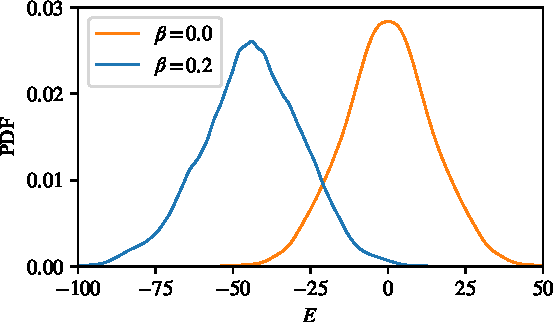
\includegraphics[width=0.6\linewidth]{ch3/energy_hist.pdf}
\caption[Distribution of energy for Ising model at different temperatures]{
Distribution of energy for the Ising model on the $10 \times 10$ square lattice at inverse temperatures $\beta = 0$ (uniform distribution) and $0.2$ (Boltzmann distribution with moderately high temperature).
The typical energies from the two distributions have a difference of around $-50$, and for larger systems and lower temperatures the difference will be even larger, which leads to exponentially low acceptance probability.
The probability density function (PDF) of the distribution is estimated from the samples using Silverman’s method~\cite{silverman1986density}.
}
\label{fig:energy-hist}
\end{figure}

Intuitively, the autocorrelation time takes two factors into account that affect the sample diversity: the correlation between the proposed configuration and the current one, and the acceptance probability. For single-spin updates, the successive samples are almost fully correlated, which leads to high autocorrelation in the observable values. On the other extreme, if we do global updates, i.e., randomly generate a proposed configuration $\vs'$ from the uniform distribution of all configurations in each sampling step, then it is fully uncorrelated with the current one. However, the energy $H(\vs')$ from the uniform distribution is almost always much higher than the current one from the target distribution, as shown in \cref{fig:energy-hist}, which makes the acceptance probability exponentially low, and the collected samples are still fully correlated. Between the two extremes of single-spin updates and global updates, a variety of cluster updates have been proposed to balance these two factors, which we will discuss in \cref{sec:cluster}.

The loss in sample diversity is reflected quantitatively in the variance of the Monte Carlo estimator in \cref{eq:monte-carlo-var}. When the Markov chain is in equilibrium, in the presence of autocorrelation, the variance increases to
\begin{equation}
\Var\big[ \bbE_\text{MCMC}[O] \big] = \frac{1}{M_{\text{eff}\,\tau}} \Var[\bar{O}],
\end{equation}
where the effective sample size
\begin{equation}
M_{\text{eff}\,\tau} = \frac{1}{2 \tau + 1} M
\end{equation}
is less than the original sample size $M$.

In many-body systems, the autocorrelation time particularly depends on the physical parameters, such as the inverse temperature $\beta$. It is a long-standing issue to MCMC that the autocorrelation time significantly increases when the system is around its critical point, know as critical slowing down~\cite{goodman1989multigrid, wolff1990critical}. Intuitively, the collective dynamics of the spins in the system can form clusters, which separate from each other by domain walls, and their average diameter is roughly the correlation length $\xi$ of the system. In the case of single-spin update, the Markov chain can be interpreted as a random walk in the configuration space, where it moves from one configuration to an adjacent one with a spin flipped. The time $\tau$ to walk the distance $\xi$ scales by $\tau \sim \xi^2$, regardless of the spatial dimension. Detailed analysis from lattice field theory has shown that $\tau \sim \xi^z$, where $z$ is the dynamical critical exponent, and $d \approx 2$ in many cases~\cite{hohenberg1977theory}. At the critical point, $\xi$ diverges until it is bounded by the system size~\cite{lubetzky2012critical}. From the perspective of statistical complexity~\cite{lopez1995statistical}, the Boltzmann distribution at the critical temperature is hard to sample from because it has both low entropy and uniformity, which lead to high complexity. It is between the high-temperature distribution with low uniformity but high entropy, and the low-temperature distribution with low entropy but high uniformity. This phenomenon proposes challenge to studies on phase transitions using MCMC, and can be alleviated by cluster updates.
\todo{A plot showing the clusters and the correlation length}

\section{Burn-in and Gelman--Rubin statistic}

The autocorrelation time $\tau$ is an important metric for the effectiveness of an MCMC algorithm when the Markov chain is already in equilibrium. However, at the beginning of MCMC, the configuration is usually initialized ``randomly'', which is from the uniform distribution of all configurations. The Markov chain can take many steps to transition from the initial configuration to a typical one in the target distribution, and these steps are called the burn-in or warm-up stage. The untypical samples in this stage introduce bias in the estimation of observables, so we need to discard them and start collecting actual samples after this stage. In theory, the length of the burn-in stage is at most on the order of magnitude of $\tau$, which lets the new configuration decorrelate with the initial one, but in practice we can estimate $\tau$ only if we already know that the burn-in stage has ended. Therefore, we need another metric to estimate the length of the burn-in stage before collecting samples from the equilibrium distribution, which can only be derived from dynamical properties of the Markov chain.
\todo{A plot showing the convergence of multiple Markov chains}

The Gelman--Rubin (GR) statistic~\cite{gelman1992inference, vats2021revisiting} can be used to identify whether the Markov chain has reached the equilibrium. To compute the GR statistic, we generate multiple independent Markov chains starting from different random initial configurations, which is a common practice to utilize the parallelization capability of modern computers~\cite{lee2010utility}. The samples are denoted by $\vs^{(j, m)}$, where $j \in [1, J]$ identifies the chain and $m \in [1, M]$ identifies the sampling step, and the corresponding observable values are denoted by $O_{j, m} = O\left( \vs^{(j, m)} \right)$. Then we have
\begin{align}
\bar{O}_j &= \frac{1}{M} \sum_{m = 1}^M O_{j, m}, \\
\bar{O}_* &= \frac{1}{J} \sum_{j = 1}^J \bar{O}_j, \\
s^2_j &= \frac{1}{M - 1} \sum_{m = 1}^M (O_{j, m} - \bar{O}_j)^2, \\
s^2_* &= \frac{1}{J} \sum_{j = 1}^J W_j,
\end{align}
where $\bar{O}_j$ is the sample mean of the observable over a chain, $\bar{O}_*$ is the sample mean of all chains, $s^2_j$ is the sample variance of a chain, and $s^2_*$ is the mean of these sample variances. Due to the presence of autocorrelation, each $s^2_j$ underestimates the true variance of the target distribution $\sigma^2$. A correction to this bias is estimated by comparing the means of different chains:
\begin{equation}
\frac{B}{M} = \frac{1}{J - 1} \sum_{j = 1}^J (\bar{O}_j - \bar{O}_*)^2.
\end{equation}
Now the estimated variance is
\begin{equation}
\sigma^2_* = \frac{M - 1}{M} s^2_* + \frac{B}{M}.
\end{equation}
The GR statistic is defined to normalize the correction to the estimated variance:
\begin{equation}
R = \sqrt{\frac{\sigma^2_*}{s^2_*}}.
\end{equation}
It is also related to the effective sample size by
\begin{equation}
R \approx \sqrt{1 + \frac{M}{M_\text{eff}}}.
\end{equation}
If we have enough random initial configurations that generate Markov chains to cover all regions of interest in the configuration space, known as the ``modes'', and they converge to similar distributions with mean observable values close to each other, we can assume that the Markov chains have reached equilibrium. It was originally proposed in Ref.~\cite{gelman1992inference} to use a threshold $R < \delta$, and a common choice is $\delta = 1.1$. According to Ref.~\cite{vats2021revisiting}, practical choices of $\delta$ ranges from $1.003$ to $1.3$, and a more stable estimation of the true variance can be obtained from batch-wise variances in the chains.

\section{Importance sampling}
\label{sec:importance-sampling}

Apart from exactly sampling the target distribution $p(\vs)$, and the MCMC sampling, there are other sampling methods to estimate the observable in \cref{eq:cl-obs}. In general, we can generate samples $\{\vs^{(1)}, \vs^{(2)}, \ldots, \vs^{(M)}\}$ from any distribution $q(\vs)$, and estimate the observable by
\begin{align}
\bbE_\text{imp}[O] &= \frac{\sum_{i = 1}^M w\left( \vs^{(i)} \right) O\left( \vs^{(i)} \right)}{\sum_{i = 1}^M w\left( \vs^{(i)} \right)}, \label{eq:importance-sampling} \\
w\left( \vs^{(i)} \right) &= \frac{p\left( \vs^{(i)} \right)}{q\left(\vs^{(i)} \right)},
\end{align}
given that $q(\vs)$ has a wider support than $p(\vs)$, i.e., $q(\vs) > 0$ for all $\vs$ such that $p(\vs) > 0$. This method is called importance sampling in statistics~\cite{kloek1978bayesian, bugallo2017adaptive}. The distribution $q(\vs)$ is also called an ``ansatz'' in the context of statistical physics. It should be close to $p(\vs)$, and easier to sample from than $p(\vs)$. Some choices of the ansatz for importance sampling will be discussed in \cref{sec:ansatz}. The variance of this estimator is
\begin{equation}
\Var\big[ \bbE_\text{imp}[O] \big] = \frac{1}{M_{\text{eff}\,w}} \Var[\bar{O}],
\label{eq:importance-sampling-var}
\end{equation}
where the effective sample size
\begin{equation}
M_{\text{eff}\,w} = \frac{\left( \sum_{i = 1}^M w\left( \vs^{(i)} \right) \right)^2}{\sum_{i = 1}^M w^2\left( \vs^{(i)} \right)}.
\end{equation}
The variance reaches its minimum when $q(\vs) = p(\vs)$, so we need to choose a $q(\vs)$ that is as close to $p(\vs)$ as possible.

However, \cref{eq:importance-sampling} generally requires to evaluate the probability $p(\vs)$, including the normalization, which is intractable for many-body systems. A more practical method is to use importance sampling with the Metropolis--Hastings algorithm in \cref{eq:metropolis}~\cite{liesenfeld2008improving, schuster2020markov}. The proposed configuration is generated from $q(\vs')$ and independent of the current configuration $\vs$, i.e., the proposal distribution $g(\vs' \mid \vs) = q(\vs')$. Then the acceptance probability becomes
\begin{equation}
A(\vs \to \vs') = \min\left( 1, \frac{p(\vs') q(\vs)}{p(\vs) q(\vs')} \right),
\label{eq:mcmc-importance}
\end{equation}
With a $q(\vs)$ that is close to $p(\vs)$, it increases the acceptance probability, while also reducing the correlation between $\vs$ and $\vs'$ compared to the single-spin update, which leads to the overall reduction of the autocorrelation time. There are more advanced methods to construct the proposal distribution that depends on the current configuration $\vs$, such as the Langevin Monte Carlo~\cite{rossky1978brownian} and the Hamiltonian Monte Carlo~\cite{duane1987hybrid}.

\section{Cluster updates}
\label{sec:cluster}

A variety of cluster update algorithms can also be discussed in the framework of MCMC importance sampling, which usually arise from studies on the percolation transition in statistical physics and graph theory, or the series expansion of the partition function~\cite{fortuin1972random, leung1991percolation, evertz1993cluster}. A prominent example is the Wolff algorithm~\cite{wolff1989collective} for the Ising model with two-body interactions. In each sampling step, it constructs a cluster of spins and flips it, such that $g(\vs' \mid \vs) \propto p_\text{B}(\vs')$, and the acceptance probability is always $1$.
\todo{Elaborate}

\dwcomment{Maybe discuss parallel tempering if there is spare time and space, but it's not used anywhere else in this thesis}

\section{Mode collapse}

Even if we collect effectively independent samples according to the autocorrelation time and the Gelman--Rubin statistic, it can still be questionable whether those samples actually represent the entire target distribution. The target distribution can have multiple modes, where a ``mode'' is defined to be a cluster of configurations $\{\vs_1, \vs_2, \vs_3, \ldots\}$ with high target probabilities $p(\vs_i)$ and high Markov transition probabilities $M_{\vs_j \vs_i}$ in \cref{eq:markov-matrix} between each other. The paths of configurations to transition from one mode to another always encounter energy barriers whose heights are proportional to the system size, so the probability of visiting different modes is exponentially low. A possible failure of MCMC is the mode collapse, where the Markov chain is seemingly in equilibrium, but actually it is only in ``equilibrium'' within a mode, and it takes an impractically long time to visit another mode, which leads to bias in the estimation of observables.

Intuitively, a mode is a peak of the target distribution in the configuration space. Although the exponentially high-dimensional configuration space cannot be directly visualized, different modes can be characterized by appropriate observables, such as the energy or the magnetization, and displayed as different peaks on the histogram of the observable. When the mode collapse happens, the estimated observable characterizing the uncovered modes becomes biased. A typical example is the two modes around the two degenerate ground states $\vs = (+1, +1, +1, \ldots)$ and $\vs = (-1, -1, -1, \ldots)$ in the ferromagnetic Ising model. In this case, even if the estimated energy is still close to the true value in a single mode, the magnetization becomes biased.
\todo{A plot of magnetization vs sampling steps}

The mode collapse in the simple case above can be eliminated by applying the spin flipping symmetry to the generated samples. Other symmetries of the Hamiltonian, such as translations and reflections, are also useful to alleviate the mode collapse and improve the accuracy of the estimated observables in general. Cluster updates are another approach to alleviate this problem, as they can propose large updates to the configuration to transition through the energy barriers that block local updates. The problem becomes more complicated in frustrated models, where the number of degenerate ground states can be exponentially large, and cannot be eliminated by a polynomially large symmetry group.
\todo{Cite some works on combinatorial optimization}

The effect of mode collapse is also demonstrated in the context of importance sampling in \cref{eq:importance-sampling}. Assuming the actual distribution of samples $q(\vs)$ only covers a single mode, and is exponentially suppressed in the uncovered modes, where $p(\vs) > 0$ but $q(\vs) \to 0$. Then we have pathologically high $w(\vs)$ in the uncovered modes, which cause the variance in \cref{eq:importance-sampling-var} to blow up. Even if an estimated observable is still close to the true value in a single mode, the blowing up variance indicates that such estimation is unreliable.

\begin{figure}[htb]
\centering
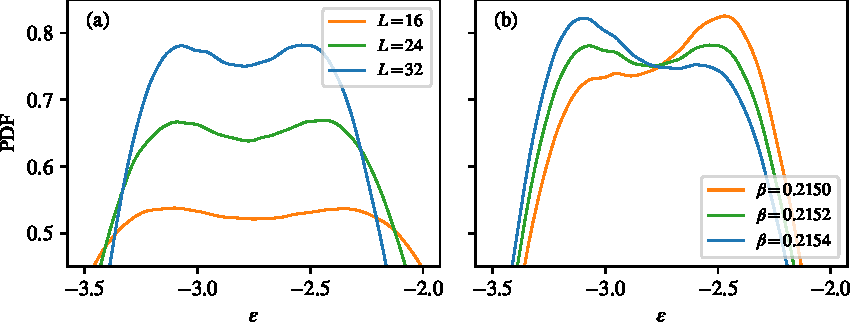
\includegraphics[width=\linewidth]{ch3/fpm_hist_p.pdf}
\caption[Distribution of energy for frustrated plaquette model]{
Distribution of the energy per site $\epsilon$ for the frustrated plaquette model (FPM) in \cref{eq:fpm}.
(a) The results with different system sizes at their respective phase transition temperatures.
(b) The results at different temperatures with the system size $L = 32$.
The probability density function (PDF) of the distribution is estimated from the samples using Silverman’s method~\cite{silverman1986density}.
The panel (a) is reproduced from Fig.~5 in Ref.~\cite{wu2021unbiased}.
}
\label{fig:fpm-hist-p}
\end{figure}

A particular consequence of mode collapse is the difficulty of MCMC sampling around first-order phase transitions of many-body systems. The first-order phase transition is characterized by a discontinuity in the energy. As an example, we investigate the transition between the ferrimagnetic (fM) and the paramagnetic (PM) phases in the 2D frustrated plaquette model (FPM) with $N = L \times L$ spins in \cref{eq:fpm}. When we plot its distribution of energies in \cref{fig:fpm-hist-p}, we can see two peaks appearing around the transition temperature. As shown in the panel (a), the depth of the valley between the two peaks grows as the system size $L$ increases, which indicates an increasing energy barrier that blocks local updates. Compared to the peak on the left, the one on the right contains more excited states, but each has lower probability, so the volumes of the two peaks are comparable. When the temperature increases, the low-energy peak shrinks while the high-energy one grows, as shown in the panel (b). The first-order phase transition appears when the two peaks happen to have the same volume. In the thermodynamic limit, the probability distribution is exponentially concentrated at the largest peak, so a change of the largest peak causes a discontinuity in the mean energy. This two-peak distribution proposes challenge to MCMC with local updates, and cluster updates are a viable approach to this problem, as we will discuss in \cref{sec:ncus}.

\chapter{Variational method}

Although MCMC is widely used to compute various observables, a limitation is that it is agnostic of the partition function $Z$ in \cref{eq:boltzmann}, therefore it cannot compute quantities that require $Z$ or the probabilities $p_\text{B}(\vs)$, including the free energy and the entropy. There are variants of MCMC designed to compute $Z$, such as the Wang--Landau algorithm~\cite{wang2001efficient, landau2021guide5}, but they involve other issues such as the discretization of the energy histogram~\cite{belardinelli2007wang}.

A different approach is to track the probability distribution in the framework of variational inference~\cite{jordan1999introduction, mackay2003information}, which also has deep roots in statistical physics starting from mean-field theories~\cite{chaikin1995principles4, zdeborova2016statistical}. We define a trial distribution $q(\vs)$, or the ``ansatz'' in the context of statistical physics, to approximate the target distribution $p(\vs)$. The form of the ansatz is chosen such that the probability $q(\vs)$ can be computed given a configuration $\vs$, and it can be easier to sample from than $p(\vs)$, or even be analytically summed over in \cref{eq:cl-obs}. Some choices of the ansatz for variational inference will be discussed in \cref{sec:ansatz}.

To make a good approximation, we want $q(\vs)$ to be as close to $p(\vs)$ as possible. A natural metric of the distance between two distributions is the Kullback--Leibler (KL) divergence~\cite{kullback1951information}:
\begin{equation}
D_\text{KL}(q \mid\mid p) = \sum_\vs q(\vs) \ln \frac{q(\vs)}{p(\vs)}.
\end{equation}
When $p(\vs)$ is the Boltzmann distribution, we have
\begin{align}
D_\text{KL}(q \mid\mid p_\text{B}) &= \sum_\vs q(\vs) \left( \ln q(\vs) - \ln \frac{\rme^{-\beta H(\vs)}}{Z} \right) \\
&= \beta (F_q - F),
\label{eq:kl-fq}
\end{align}
where $F = -\frac{1}{\beta} \ln Z$ is the true free energy, and we define the variational free energy
\begin{equation}
F_q = \sum_\vs q(\vs) F_{q\,\text{loc}}(\vs),
\label{eq:fq}
\end{equation}
and the local free energy
\begin{equation}
F_{q\,\text{loc}}(\vs) = \frac{1}{\beta} \ln q(\vs) + H(\vs).
\label{eq:fq-loc}
\end{equation}

Like how we have approximated \cref{eq:cl-obs} by \cref{eq:monte-carlo}, the variational free energy in \cref{eq:fq} is also a weighted summation over the distribution $q(\vs)$ with exponentially many terms, and we can estimate it by Monte Carlo sampling:
\begin{equation}
\bbE_\text{MC}[F_q] = \frac{1}{M} \sum_{i = 1}^M F_{q\,\text{loc}}\left( \vs^{(i)} \right), \quad
\vs^{(i)} \sim q.
\label{eq:fq-monte-carlo}
\end{equation}
We refer to this method as variational Monte Carlo (VMC). Although the term VMC is mostly discussed in the context of quantum problems, as we will see through this thesis, the setting of VMC for classical problems is analogous to the quantum one. There is a difference from MCMC, though, that the variational inference of \cref{eq:fq-loc} requires to evaluate the probability $q(\vs)$, including the normalization, even if the normalization constant cancels out in the derivation of the Markov Chain in \cref{eq:metropolis}. Therefore, it is important to choose an ansatz $q(\vs)$ whose probability can be computed efficiently.
\todo{Before neural networks, what ansatzes were used in classical problems that require Monte Carlo sampling rather than analytical study?}

The ansatz $q(\vs)$ can be a set of distributions defined by some tunable parameters $\theta$, and we vary $\theta$ to minimize the KL divergence. In \cref{eq:kl-fq}, $F$ is independent of $\theta$, so we only need to minimize $F_q$. As the KL divergence is non-negative, the lower bond of $F_q$ is exactly the true free energy $F$, which is desired to compute in many cases. In practice, the target of minimization is $\beta F_q$ rather than $F_q$ itself, to avoid the singularity of $\frac{1}{\beta}$ in \cref{eq:fq} when $\beta \to 0$.

As $F_q$ is generally a multivariate nonlinear function of $\theta$, its optimization is usually performed by gradient descent (GD)-based algorithms~\cite{curry1944method}. In the most naive setting of GD, in each optimization step $t$ we update $\theta$ by
\begin{equation}
\theta_{t + 1} \gets \theta_t - \gamma \left.\frac{\partial F_q}{\partial \theta}\right|_{\theta = \theta_t},
\label{eq:gd}
\end{equation}
where $\gamma$ is a small positive number called the learning rate. A common challenge in GD is to choose an appropriate magnitude of $\gamma$, such that the optimization is stable while converges in reasonably few steps~\cite{boyd2004convex}. Another challenge is to converge to the global minimum without being trapped by local minima and saddle points, which is of most interest in physics. In the recent trend of machine learning, many advanced variants of GD have been proposed.
\todo{Discuss the optimizers somewhere}

In modern software, the gradient $\frac{\partial F_q}{\partial \theta}$ in \cref{eq:gd} is derived by automatic differentiation~\cite{baydin2018automatic}, which can be more stable and efficient than traditional methods of finite difference, and more error-prone than manually deriving and implementing the gradient. Care should be taken that \cref{eq:fq} involves the distribution $q(\vs)$, which is a function of $\theta$, but this term no longer exists after replacing \cref{eq:fq} by \cref{eq:fq-monte-carlo}, and we cannot take the gradient of probabilities of the configurations in the usual way after sampling the configurations when evaluating \cref{eq:fq-monte-carlo}. Therefore, we rewrite the gradient of \cref{eq:fq} by
\begin{align}
\frac{\partial F_q}{\partial \theta}
&= \sum_\vs \left( \frac{\partial q(\vs)}{\partial \theta} F_{q\,\text{loc}}(\vs) + q(\vs) \frac{\partial F_{q\,\text{loc}}(\vs)}{\partial \theta} \right) \\
&= \sum_\vs \left( q(\vs) \frac{\partial \ln q(\vs)}{\partial \theta} F_{q\,\text{loc}}(\vs) + q(\vs) \frac{1}{\beta} \frac{\partial \ln q(\vs)}{\partial \theta} \right).
\label{eq:fq-grad-2-terms}
\end{align}
The second term of \cref{eq:fq-grad-2-terms} becomes
\begin{align}
\frac{1}{\beta} \sum_\vs q(\vs) \frac{\partial \ln q(\vs)}{\partial \theta}
&= \frac{1}{\beta} \sum_\vs \frac{\partial q(\vs)}{\partial \theta} \\
&= \frac{1}{\beta} \frac{\partial}{\partial \theta} \sum_\vs q(\vs) \\
&= \frac{1}{\beta} \frac{\partial}{\partial \theta} 1 \\
&= 0,
\end{align}
as $q(\vs)$ is normalized. The remaining first term of \cref{eq:fq-grad-2-terms} can be again estimated by Monte Carlo sampling:
\begin{equation}
\bbE_\text{MC}\left[ \frac{\partial F_q}{\partial \theta} \right]
= \frac{1}{M} \sum_{i = 1}^M F_{q\,\text{loc}}\left( \vs^{(i)} \right) \frac{\partial \ln q\left( \vs^{(i)} \right)}{\partial \theta}, \quad
\vs^{(i)} \sim q.
\label{eq:fq-grad}
\end{equation}
This method is called the REINFORCE gradient~\cite{williams1992simple} or the policy gradient~\cite{sutton1999policy} in the context of machine learning, and the gradient of the log-probability $\frac{\partial \ln q(\vs)}{\partial \theta}$ is called the score function~\cite{fisher1935detection, hyvarinen2005estimation}. This kind of differentiation through discrete variables and stochastic sampling of distributions is a recent interest in automatic differentiation frameworks~\cite{krieken2021storchastic, arya2022automatic, catumba2023stochastic}.
\todo{Discuss variance reduction?}

\chapter{Ansatzes for the Boltzmann distribution}
\label{sec:ansatz}

In the following, we discuss some choices of the ansatz to approximate the Boltzmann distribution.

\section{Naive mean-field ansatz}

An early practice of mean-field theory, known as the Curie--Weiss model~\cite{weiss1907hypothese, nishimori2001statistical}, was proposed to study the phase transition of the classical Ising model. Here we recapitulate its derivation and reformulate it in the framework of variational ansatzes.

The Hamiltonian in \cref{eq:cl-ising} can be written as the sum of each spin $s_i$ in its local magnetic field $h_{\text{loc}\,i}$ produced by adjacent spins:
\begin{align}
H(\vs) &= J \sum_{\langle i, j \rangle} s_i s_j
= \frac{1}{2} J \sum_i h_{\text{loc}\,i} s_i, \\
h_{\text{loc}\,i} &= \sum_{j \in \partial i} s_j,
\end{align}
where $\partial i$ denotes the set of nearest neighbors of the site $i$. To find an ansatz whose free energy can be analytically studied, we start from replacing $h_{\text{loc}\,i}$ by an approximate mean field produced by all spins:
\begin{equation}
h_{\text{loc}\,i} \approx h_\text{MF} = \frac{2 d}{N} \sum_i s_i,
\end{equation}
where $d$ is the average number of nearest neighbors per site, and each site has $2 d$ nearest neighbors. Then the locally interacting model becomes a globally interacting mean-field model
\begin{equation}
H(\vs) \approx H_\text{MF}(\vs) = \frac{d J}{N} \sum_{i, j} s_i s_j.
\label{eq:ham-mf}
\end{equation}

Next, we split each spin variable into $s_i = m + \delta s_i$, where $m$ is the mean magnetization, $\delta s_i$ is the fluctuation around the mean, and we assume $|\delta s_i| \ll |m|$. Then \cref{eq:ham-mf} becomes
\begin{align}
H_\text{MF}(\vs) &= \frac{d J}{N} \sum_{i, j} (m + \delta s_i) (m + \delta s_j) \\
&= d J m \sum_i (m + 2 \delta s_i) + \calO(\delta s^2) \\
&= d J m \sum_i (2 s_i - m) + \calO(\delta s^2).
\end{align}
Ignoring the higher-order terms $\calO(\delta s^2)$, the mean-field model can be written in a non-interacting form:
\begin{align}
H_\text{MF}(\vs) &= \sum_i H_{\text{MF}\,i}(s_i), \\
H_{\text{MF}\,i}(s_i) &= d J m (2 s_i - m).
\label{eq:ham-mf-noninter}
\end{align}
Thus we can perform the summation of the partition function:
\begin{equation}
Z_\text{MF}
% = \sum_\vs \rme^{-\beta H_\text{MF}(\vs)}
= \left( \sum_s \rme^{-\beta H_{\text{MF}\,i}(s)} \right)^N
= \left( \rme^{d \beta J m^2} \cdot 2 \cosh (2 d \beta J m) \right)^N.
\end{equation}
The free energy is
\begin{equation}
F_\text{MF} = -\frac{1}{\beta} \ln Z_\text{MF} = - \frac{N}{\beta} \left(d \beta J m^2 + \ln \left( 2 \cosh (2 d \beta J m) \right) \right).
\label{eq:fe-mf}
\end{equation}

At this point, the mean-field free energy $F_\text{MF}$ is derived from the approximated Hamiltonian in \cref{eq:ham-mf}, and we have no guarantee that it is an upper bound of the true free energy derived from the original Hamiltonian in \cref{eq:cl-ising}. However, \cref{eq:kl-fq} still motivates us to minimize $F_\text{MF}$, and the tunable parameter $\theta$ is $m$ here. When $F_\text{MF}$ reaches its minimum, we have the self-consistent equation
\begin{equation}
\frac{\partial F_\text{MF}}{\partial m} = 0 \implies
m + \tanh(2 d \beta J m) = 0.
\label{eq:cw}
\end{equation}
\Cref{eq:cw} has non-zero solutions only when $2 d \beta J < -1$, where $J < 0$ and the critical temperature $T_\text{c} = \frac{1}{\beta_\text{c}} = 2 d (-J)$. Therefore, at low temperatures $T < T_c$, the system is ferromagnetic with spontaneous magnetization as the non-zero solutions of \cref{eq:cw}; otherwise, at high temperatures $T > T_c$, the system is paramagnetic without spontaneous magnetization.
\todo{A plot of \cref{eq:cw}}

The non-interacting Hamiltonian \cref{eq:ham-mf-noninter} also implies that the joint probability $p(\vs)$ can be factorized into univariate probabilities:
\begin{align}
p_\text{MF}(\vs) &= \prod_i p_{\text{MF}\,i}(s_i), \\
p_{\text{MF}\,i}(s_i) &= \frac{\rme^{-\beta H_{\text{MF}\,i}(s_i)}}{\sum_s \rme^{-\beta H_{\text{MF}\,i}(s)}}.
\end{align}
Simplifying $p_\text{MF}(s_i)$ with \cref{eq:cw}, we have
\begin{equation}
p_\spinup = p_{\text{MF}\,i}(s_i = +1) = \frac{1 + m}{2}, \quad
p_\spindown = p_{\text{MF}\,i}(s_i = -1) = \frac{1 - m}{2}.
\label{eq:p-mf}
\end{equation}
The probability distribution $p_\text{MF}(\vs)$ can serve as a variational ansatz with a single tunable parameter $m$, which we refer to as the naive mean-field (NMF) ansatz.

Next, we use the NMF ansatz and the original Hamiltonian in \cref{eq:cl-ising} to evaluate the variational energy. The energy can be directly evaluated by
\begin{align}
E_\text{MF} &= \sum_\vs p_\text{MF}(\vs) H(\vs) \\
&= N d J (p_\spinup p_\spinup - p_\spinup p_\spindown - p_\spindown p_\spinup + p_\spindown p_\spindown) \\
&= N d J m^2, \\
\shortintertext{and the entropy is}
S_\text{MF} &= -\sum_\vs p_\text{MF}(\vs) \ln p_\text{MF}(\vs) \\
&= -N (p_\spinup \ln p_\spinup + p_\spindown \ln p_\spindown).
\end{align}
Under this ansatz, the free energy $F_\text{MF} = E_\text{MF} - \frac{1}{\beta} S_\text{MF}$ is the same as \cref{eq:fe-mf} derived from the approximated Hamiltonian. It is an upper bound of the true free energy, as it is now derived from the original Hamiltonian. For more complicated models on non-regular graphs and with more than two-body interactions, were \cref{eq:cw} is not directly applicable, we can still apply the NMF ansatz to obtain a preliminary variational approximation.

\section{Bethe ansatz}

Starting from an analytical solution to the 1D quantum Heisenberg model~\cite{bethe1931theorie}, the Bethe ansatz has become a gross term for methods to exactly solve~\cite{baxter1995solvable, caravelli2022some} or approximate partition functions on lattices and other graphs~\cite{gujrati1995bethe, mezard2001bethe}. It is also deeply related to the belief propagation, a message passing algorithm used in Bayesian inference and the recent trend of graph machine learning~\cite{yedidia2003understanding, ikeda2004stochastic}. Unlike the NMF ansatz which approximates the original model using only uniform global interactions, the Bethe ansatz utilizes the local geometry to more accurately evaluate interactions between nearest neighbors.

In general, the Bethe ansatz is applicable to a probability distribution defined on a graph $\calG = (\calV, \calE)$, where $\calV$ is the set of sites and $\calE$ is the set of edges, and the probability of each configuration can be factorized into two-body interactions:
\begin{equation}
p(\vs) = \frac{1}{Z} \prod_{(i, j) \in \calE} f_{i j}(s_i, s_j).
\end{equation}
For the Ising model in \cref{eq:cl-ising}, we have
\begin{equation}
f_{i j}(s_i, s_j) = \rme^{-\beta J s_i s_j}.
\end{equation}
To study the properties of an edge or a site while marginalizing the rest of the graph, we define the auxiliary probability with an edge $(i j)$ removed from the graph:
\begin{align}
\mu^{(i j)}(\vs) &= \frac{1}{Z^{(i j)}} \prod_{(k, l) \in \calE \setminus (i j)} f_{k l}(s_k, s_l), \\
\shortintertext{and with all edges on the site $i$ removed from the graph:}
\mu^{(i)}(\vs) &= \frac{1}{Z^{(i)}} \prod_{(k, l) \in \calE, i \notin \{k, l\}} f_{k l}(s_k, s_l),
\end{align}
where $Z^{(i j)}$ and $Z^{(i)}$ are corresponding normalization constants. We also take the marginal probabilities
\begin{align}
\mu^{(i j)}_i(s_i) &= \sum_{\vs_{\calV \setminus i}} \mu^{(i j)}(s_i, \vs_{\calV \setminus i}), \\
\mu^{(i j)}_{i j}(s_i, s_j) &= \sum_{\vs_{\calV \setminus \{i, j\}}} \mu^{(i j)}(s_i, s_j, \vs_{\calV \setminus \{i, j\}}), \\
\mu^{(i)}_{\partial i}(\vs_{\partial i}) &= \sum_{\vs_{\calV \setminus \partial i}} \mu^{(i)}(\vs_{\partial i}, \vs_{\calV \setminus \partial i}),
\end{align}
where $\partial i = \left\{ j \mid (i, j) \in \calE \right\}$ denotes the neighbors of the site $i$. The univariate marginal probability with an edge removed is denoted by the ``message'':
\begin{equation}
\mu_{i \to j}(s_i) = \mu^{(i j)}_i(s_i).
\end{equation}
After removing the edge $(i, j)$, there is no interaction between $i$ and $j$ after marginalizing other sites, so we have
\begin{equation}
\mu^{(i j)}_{i j}(s_i, s_j) = \mu_{i \to j}(s_i) \mu_{j \to i}(s_j).
\end{equation}

Then we write down the relation between $\mu^{(i j)}(\vs)$ and $\mu^{(i)}(\vs)$. Temporarily ignoring the normalization constants, we can marginalize $\mu^{(i j)}(\vs)$ by first marginalizing $\mu^{(i)}(\vs)$ and then evaluating the remaining interactions between $i$ and $\partial i \setminus j$:
\begin{equation}
\mu^{(i j)}_{i j}(s_i, s_j) \propto \sum_{\vs_{\partial i \setminus j}} \mu^{(i)}_{\partial i}(s_j, \vs_{\partial i \setminus j}) \prod_{k \in \partial i \setminus j} f_{i k}(s_i, s_k).
\end{equation}
It is proposed to approximate $\mu^{(i)}_{\partial i}(\vs_{\partial i})$ by the messages:
\begin{equation}
\mu^{(i)}_{\partial i}(\vs_{\partial i}) \approx \prod_{j \in \partial i} \mu_{j \to i}(s_j).
\label{eq:bethe-prob}
\end{equation}
Now we have the self-consistent equations
\begin{align}
\mu_{i \to j}(s_i) &\propto \sum_{\vs_{\partial i \setminus j}} \prod_{k \in \partial i \setminus j} \mu_{k \to i}(s_k) \prod_{k \in \partial i \setminus j} f_{i k}(s_i, s_k) \\
&= \prod_{k \in \partial i \setminus j} \sum_{s_k} f_{i k}(s_i, s_k) \mu_{k \to i}(s_k),
\label{eq:bethe-message}
\end{align}
from which we can solve the $4 N d$ variables $\mu_{i \to j}(s_i)$. After recovering the normalization constants in \cref{eq:bethe-message}, they can be solved by iterative algorithms if convergence conditions are satisfied~\cite{mooij2007sufficient}, or by gradient descent-based algorithms.

Knowing the messages, we can obtain the two-body marginals of the original distribution
\begin{equation}
\mu_{i j}(s_i, s_j) = \frac{f_{i j}(s_i, s_j) \mu_{i \to j}(s_i) \mu_{j \to i}(s_j)}{\sum_{s'_i, s'_j} f_{i j}(s'_i, s'_j) \mu_{i \to j}(s'_i) \mu_{j \to i}(s'_j)},
\end{equation}
and estimate the energy and other observables with at most two-body interactions. For the Ising model in \cref{eq:cl-ising}, we have
\begin{equation}
E_\text{Bethe} = J \sum_{\langle i, j \rangle} \mu_{i j}(s_i, s_j) s_i s_j.
\end{equation}
We can also construct a Bethe entropy from the edge terms and the site terms:
\begin{align}
S_\text{Bethe} &= S_\calE + S_\calV, \\
S_\calE &= -\sum_{(i, j) \in \calE} \ln \sum_{s_i, s_j} f_{i j}(s_i, s_j) \mu_{i \to j}(s_i) \mu_{j \to i}(s_j), \\
S_\calV &= \sum_i \ln \sum_{s_i} \prod_{j \in \partial i} \sum_{s_j} f_{i j}(s_i, s_j) \mu_{j \to i}(s_j),
\end{align}
and the Bethe free energy $F_\text{Bethe} = E_\text{Bethe} - \frac{1}{\beta} S_\text{Bethe}$. The Bethe entropy is exactly the true energy when the graph is a tree, but not for general graphs. Therefore, the Bethe free energy is not guaranteed to be an upper bound of the true free energy.

\section{Neural network ansatzes}

\todo{Move some general introduction to the first chapter}

Neural networks, in the context of modern machine learning, are a diverse class of mathematical functions that are historically inspired by the functionality of biological neural networks~\cite{mackay2003information, goodfellow2016deep}. They typically have numerous parameters, where the modern large models have reached hundreds of billions of parameters~\cite{brown2020language}. In theory, they are universal approximators of any well-behaved functions if optimized w.r.t.\ the parameters~\cite{hornik1989multilayer}. Although the ideal optimization of so many parameters is intractable in practice, they can still be far more expressive than traditional function approximators~\cite{sontag1998vc}. On the other hand, the large number of parameters makes them more computationally expensive than traditional approaches, and they are usually executed on graphics processing units (GPU) or other specialized hardware~\cite{chen2020survey}. The optimization of these parameters is known as ``training'' or ``learning'', highlighting the paradigmatic difference from the traditional optimization problems with few variables.

Since their breakthrough on image classification problems~\cite{krizhevsky2012imagenet}, neural networks have opened a new era of machine learning, known as ``deep learning''~\cite{goodfellow2016deep}. They have achieved state-of-the-art results on all machine learning domains, and led to a growth of the data-driven paradigm in vast scientific fields~\cite{montans2019data}. The prominent examples including the modeling of languages~\cite{brown2020language}, images~\cite{rombach2022high}, and strategic games~\cite{silver2016mastering}. Such success is conjectured to stem from the high efficiency of neural networks to represent complicated probability distributions in exponentially high-dimensional spaces --- probabilities of valid speeches in the space of many words, probabilities of recognizable images in the space of many pixels, and probabilities of winning moves in the space of many game board states. Therefore, they have also been introduced as ansatzes in many-body physics, where the distributions are a central problem.

\todo{A figure of layers}
Neural networks are composed of a common set of functions, known as ``layers'', and the composition can be arbitrarily sophisticated. The basic architecture is the feedforward network, which is defined by a sequential composition of alternating linear layers and nonlinear activation functions:
\begin{equation}
\vy = (\text{Lin}_1 \circ \text{Act}_1 \circ \text{Lin}_2 \circ \text{Act}_2 \circ \cdots \circ \text{Lin}_{n_\text{l}} \circ \text{Act}_{n_\text{l}})(\vx),
\end{equation}
where $\vx$ is the inputs to the network, $\vy$ is the outputs, $n_\text{l}$ is the number of layers, and $\circ$ denotes function composition. The linear layer is defined by
\begin{equation}
\text{Lin}_i(\vx_i) = \mW_i \vx_i + \mb_i,
\end{equation}
where $\mW_i$ is the weight and $\mb_i$ is the bias, which are the parameters of this layer, and every layer has different parameters. Assuming $\vx_i$ is a vector of size $n_{\text{in}\,i}$, we can choose an output size $n_{\text{out}\,i}$, then $\mW_i$ is inferred to be a matrix of size $n_{\text{out}\,i} \times n_{\text{in}\,i}$, $\mb_i$ is a vector of size $n_{\text{out}\,i}$, and the input size of the next linear layer $n_{\text{in}\,i + 1}$ is $n_{\text{out}\,i}$.
In practice, the inputs $\vx_i$ have an additional batch dimension, which denotes evaluating the same network on different input samples, but it is omitted in our discussion for simplicity. The sizes of the intermediate outputs are known as the ``hidden sizes'', and the hyperparameters of the network include the number of layers and the hidden sizes. These hyperparameters, in contrast to the parameters $\mW_i$ and $\mb_i$, define the architecture of the network and mostly determine its expressiveness.

The activation function is an element-wise function of the input vector. A great variety of activation functions has been proposed, each with its own claimed advantages, but most are proved in practice to be minuscule improvements~\cite{kunc2024three}. The simplest choice is the rectified linear unit (ReLU):
\begin{equation}
\text{ReLU}(x) = \begin{cases}
x, & x > 0 \\
0, & x \leq 0
\end{cases}.
\end{equation}
It has been used since the early research on neural networks, and is still efficient today despite its simplicity. A modern choice is the Gaussian error linear unit (GELU)~\cite{hendrycks2016gaussian}:
\begin{equation}
\text{GELU}(x) = x\,\Phi(x),
\end{equation}
where $\Phi(x)$ is the cumulative distribution function (CDF) of the unit Gaussian distribution. While having the same asymptotic behaviors as ReLU, it is derived from the stochastic regularization of the network, and helps stabilize evaluation and training of the network. It is the default choice in NetKet~\cite{carleo2019netket}, and is used in most results reported in this thesis. The activation functions in the last layer can be the identity function if the outputs are unconstrained in $\bbR$, or specifically constructed to constrain the outputs in an interval. In the latter case, a common choice is the sigmoid function:
\begin{equation}
\text{Sigmoid}(x) = \frac{1}{1 + \rme^{-x}},
\end{equation}
which maps from $\bbR$ to $(0, 1)$, or to another interval with an additional linear transform.
\todo{A plot of the activation functions if we really need to take space}

Many-body systems usually have symmetries and locality, which also arise in machine learning of natural images. To take these advantages, the linear layers can be specialized into convolutional layers. Ignoring the layer index, a convolutional layer is denoted by $\vy = \text{Conv}(\vx)$, and in the 1D case it is defined by
\begin{equation}
y_{i, c} = \sum_{k = 1}^{n_\text{k}} \sum_{c' = 1}^{n_\text{c in}} W_{j, c, c'} x_{i + j - 1, c'} + b_{i, c},
\label{eq:conv-layer}
\end{equation}
where $\vx$ is an array of size $n_\text{s} \times n_\text{c in}$, $\vy$ is an array of size $n_\text{s} \times n_\text{c out}$, and we assume that the spatial dimension $n_\text{s}$ is the same in the inputs and the outputs for simplicity. Both the inputs and the outputs have another dimension of ``channels'', also known as ``features'', which determines the size of the network. The convolutional layer acts as if a linear layer on the channel dimension, mapping from $n_\text{c in}$ channels to $n_\text{c out}$ channels. Only on the spatial dimension, it performs a convolution. The weights $\mW$ is an array of size $n_\text{k} \times n_\text{c out} \times n_\text{c in}$, where $n_\text{s}$ is the convolution kernel size, and the biases $\mb$ is an array of size $n_\text{k} \times n_\text{c out}$. Higher-dimensional convolutional layers can be defined similarly. In \cref{eq:conv-layer}, care should be taken when accessing the out-of-boundary values $x_{i, c}$ where $i > n_\text{s}$. For physical systems with OBC, the common practice is padding with zeros: $x_{i, c} = 0$; while for PBC, the boundary can be correspondingly periodic: $x_{i, c} = x_{i - L, c}$.

In the PBC case, the convolutional layer is translational equivariant in the spatial dimension, which means a translation of the inputs leads to the same translation of the outputs:
\begin{equation}
T_d \text{Conv}(\vx) = \text{Conv}(T_d \vx),
\end{equation}
where $T_d$ denotes the translation by $d$ steps: $T (x_1, x_2, \ldots, x_{n_\text{s}})$ = $(x_{1 + d}, x_{2 + d}, \ldots, x_{n_\text{s}}, x_1, x_2, \ldots, x_d)$. Beyond the translational symmetry, this equivariance can be generalized to more symmetry groups such as rotations and reflections~\cite{roth2021group}.

To introduce a neural network as the ansatz for a many-body system of $N$ spins, one may naively define
\begin{align}
q_\theta(\vs) &= \frac{1}{Z} \text{NN}(\vs), \\
Z &= \sum_\vs \text{NN}(\vs),
\end{align}
where NN is a neural network with input size $N$ and a scalar output, and $\theta$ denotes all parameters in it. However, the normalization constant $Z$ is an intractable sum of exponentially many configurations, and this distribution is not easier to sample from than the Boltzmann distribution, therefore it cannot be used in MCMC importance sampling in \cref{eq:mcmc-importance} or VMC in \cref{eq:fq}.

Some early attempts have been proposed~\cite{huang2017accelerated, liu2017self} to choose a simple ansatz which allows efficient cluster updates, such as a two-body interacting Hamiltonian or a restricted Boltzmann machine (RBM), and use it in \cref{eq:mcmc-importance}. As the normalization constant of the ansatz is still intractable, and the variational inference is unavailable, the parameters of the ansatz are trained in a supervised learning approach. One first generate some samples from the target distribution using traditional MCMC, then optimize the energies of these samples evaluated by the ansatz towards those evaluated by the original Hamiltonian. After training, more samples can be generated from the ansatz using efficient cluster updates. However, the quality of the samples used in training limits the accuracy of the ansatz.

Another approach is to specifically construct a neural network with tractable probabilities. A prominent family of such approach is the autoregressive models which we will discuss in \cref{sec:arnn}. Another notable family of neural networks with this property is the normalizing flows~\cite{song2017nice, muller2019neural}, which reparameterize the target distribution into a simple one using the same principle as \cref{eq:reparam}. They are mostly used for continuous variables, thus are out of the scope of this thesis.

\dwcomment{Tensor networks are also used to generate classical distributions but let's leave them to the quantum part}
